\section{Results}\label{sec:results}

% ==================================================================
%
% EB writes here
%


\begin{figure}[H]
    \centering
    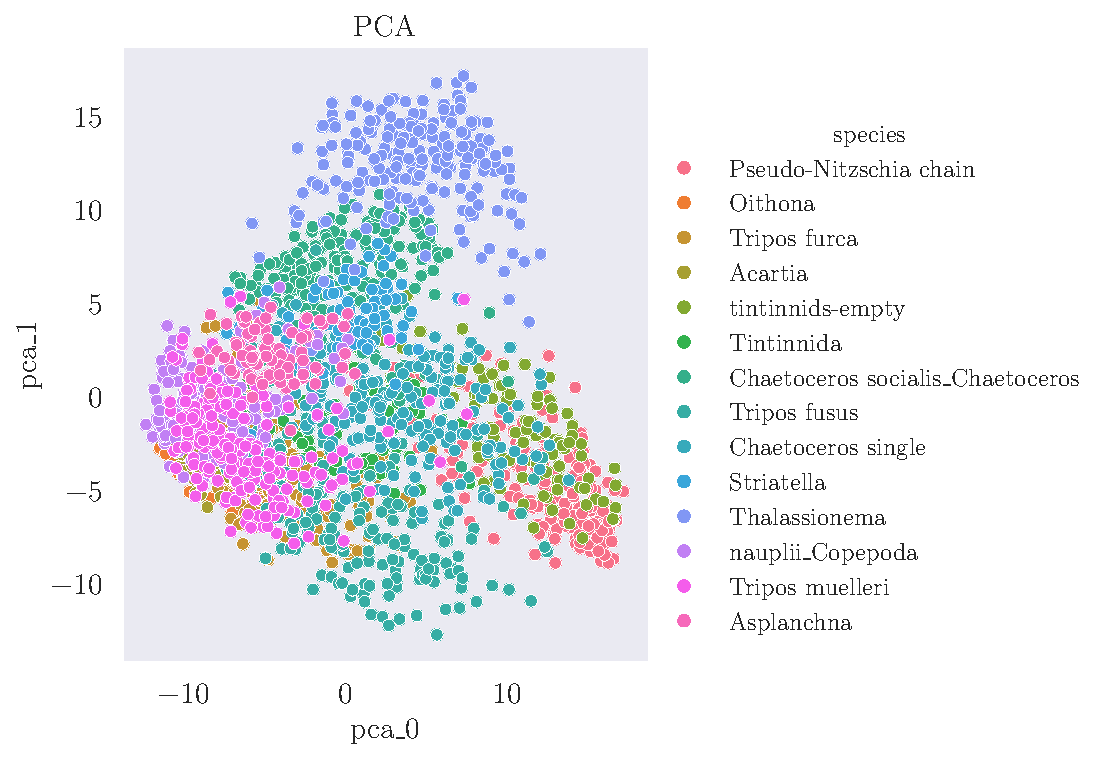
\includegraphics[width=1.1\linewidth]{examples/tests_eb/figs/pca0_pca1.pdf}
    \caption{The two first principal components out of 70 plotted against each other. Already here we can see some weak signs of clusters}
    \label{fig:pca0pca1}
\end{figure}

\begin{figure}[H]
    \centering
    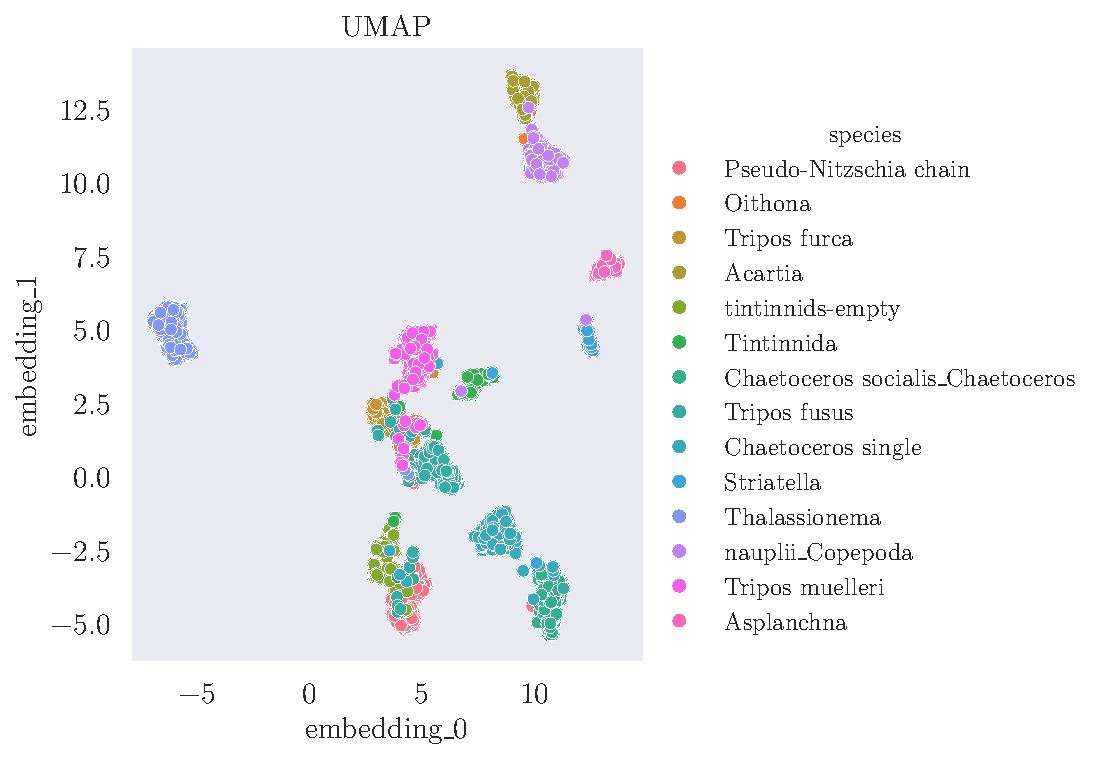
\includegraphics[width=1.1\linewidth]{examples/tests_eb/figs/umap.pdf}
    \caption{A UMAP plot to explore non-linear relations in our data (TODO - read up on UMAP). Here we can clearly see how our extracted features cluster together, yet we still do not have 14 distinct clusters.}
    \label{fig:enter-label}
\end{figure}

% ==================================================================